Grundlegend für Streuexperimente ist der Wirkungsquerschnitt $\sigma$.
Der Wirkungsquerschnitt beschreibt die Wechselwirkungswahrscheinlichkeit eines Projektils (P) mit einem Target (T).
Dabei hat $\sigma$ die Dimension einer Fläche und beschreibt anschaulich eine 'Wechselwirkungsfläche' des jeweiligen Atoms im Target.
\begin{figure}[h!]
  \centering
  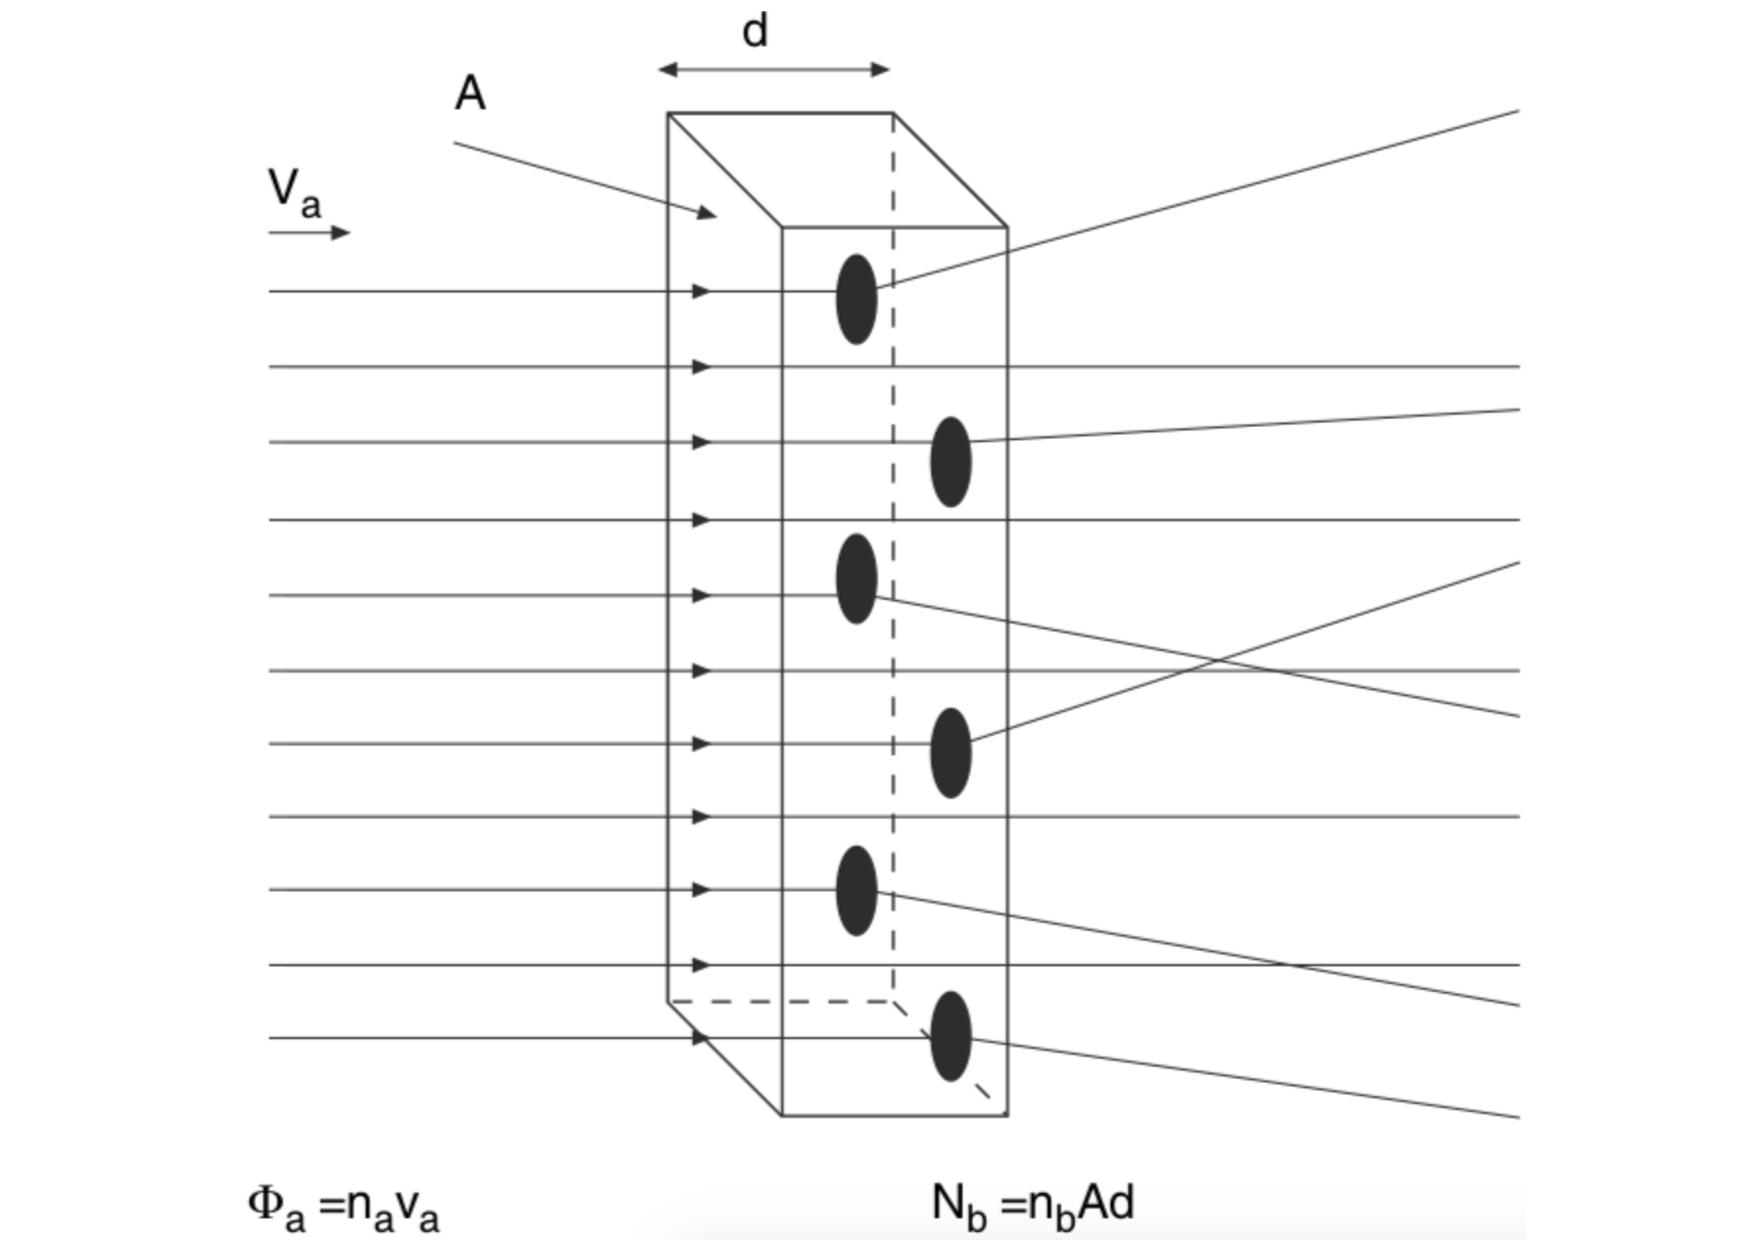
\includegraphics[width=0.4\textwidth]{images/wq.pdf}
  \caption{Anschauliche Beschreibung des Wirkungsquerschnitts $\sigma$ \cite{povh}.}
  \label{fig:wq}
\end{figure}
Je größer die Fläche, desto wahrscheinlicher die Streuung.
%
\\Die $\alpha$-Teilchen, die bei der Rutherford-Streuung verwendet werden, verlieren in der Folie ihre kinetische Energie.
Allgemein kann der Energieverlust von geladenen Teilchenstrahlen in Materie über verschiedene Prozesse entstehen.
Bei Wechselwirkung von schweren geladenen Teilchen mit der Elektronenhülle wird die Bethe-Bloch-Gleichung \eqref{eqn:bethebloch} verwendet.
\begin{equation}
	- \frac{d E}{d x} = - \frac{4 \pi e^4 z^2 N Z}{m_0 v^2 (4 \pi \epsilon_0)^2} \ln{\frac{2 m_0 v^2}{I}}
	\label{eqn:bethebloch}
\end{equation}
Hier ist $e$ die Elementarladung, $v$ die Geschwindigkeit des Projektils, $z$ die Ladungszahl des Projektils, $Z$ die Ladungszahl des Targets, $N$ die Teilchendichte im Target und $I$ das mittlere Ionisationspotenzial des Targets.
Das mittlere Ionisationspotenzial $I$ kann durch folgende Beziehung genähert werden:
\begin{equation*}
	I= \SI{10}{eV} \cdot Z.
\end{equation*}
Die Bethe-Bloch-Gleichung ist die quantenmechanische Erweiterung der klassischen Gleichung zum Energieverlust über Anregungs- und Ionisationsprozesse von Niels Bohr.
Die wesentlichen Annahmen, die hierfür getroffen werden müssen sind folgende:
\begin{enumerate}
	\item $M_{\text{T}} >> m_{\text{P}}$: Das passierende Teilchen wird nicht abgelenkt.
	\item $v_{\text{P}} >> v_{e^-} \approx 0$: Die Schalenelektronen bewegen sich während der Wechselwirkung nicht.
\end{enumerate}
%\begin{figure}[h!]
%  \centering
%  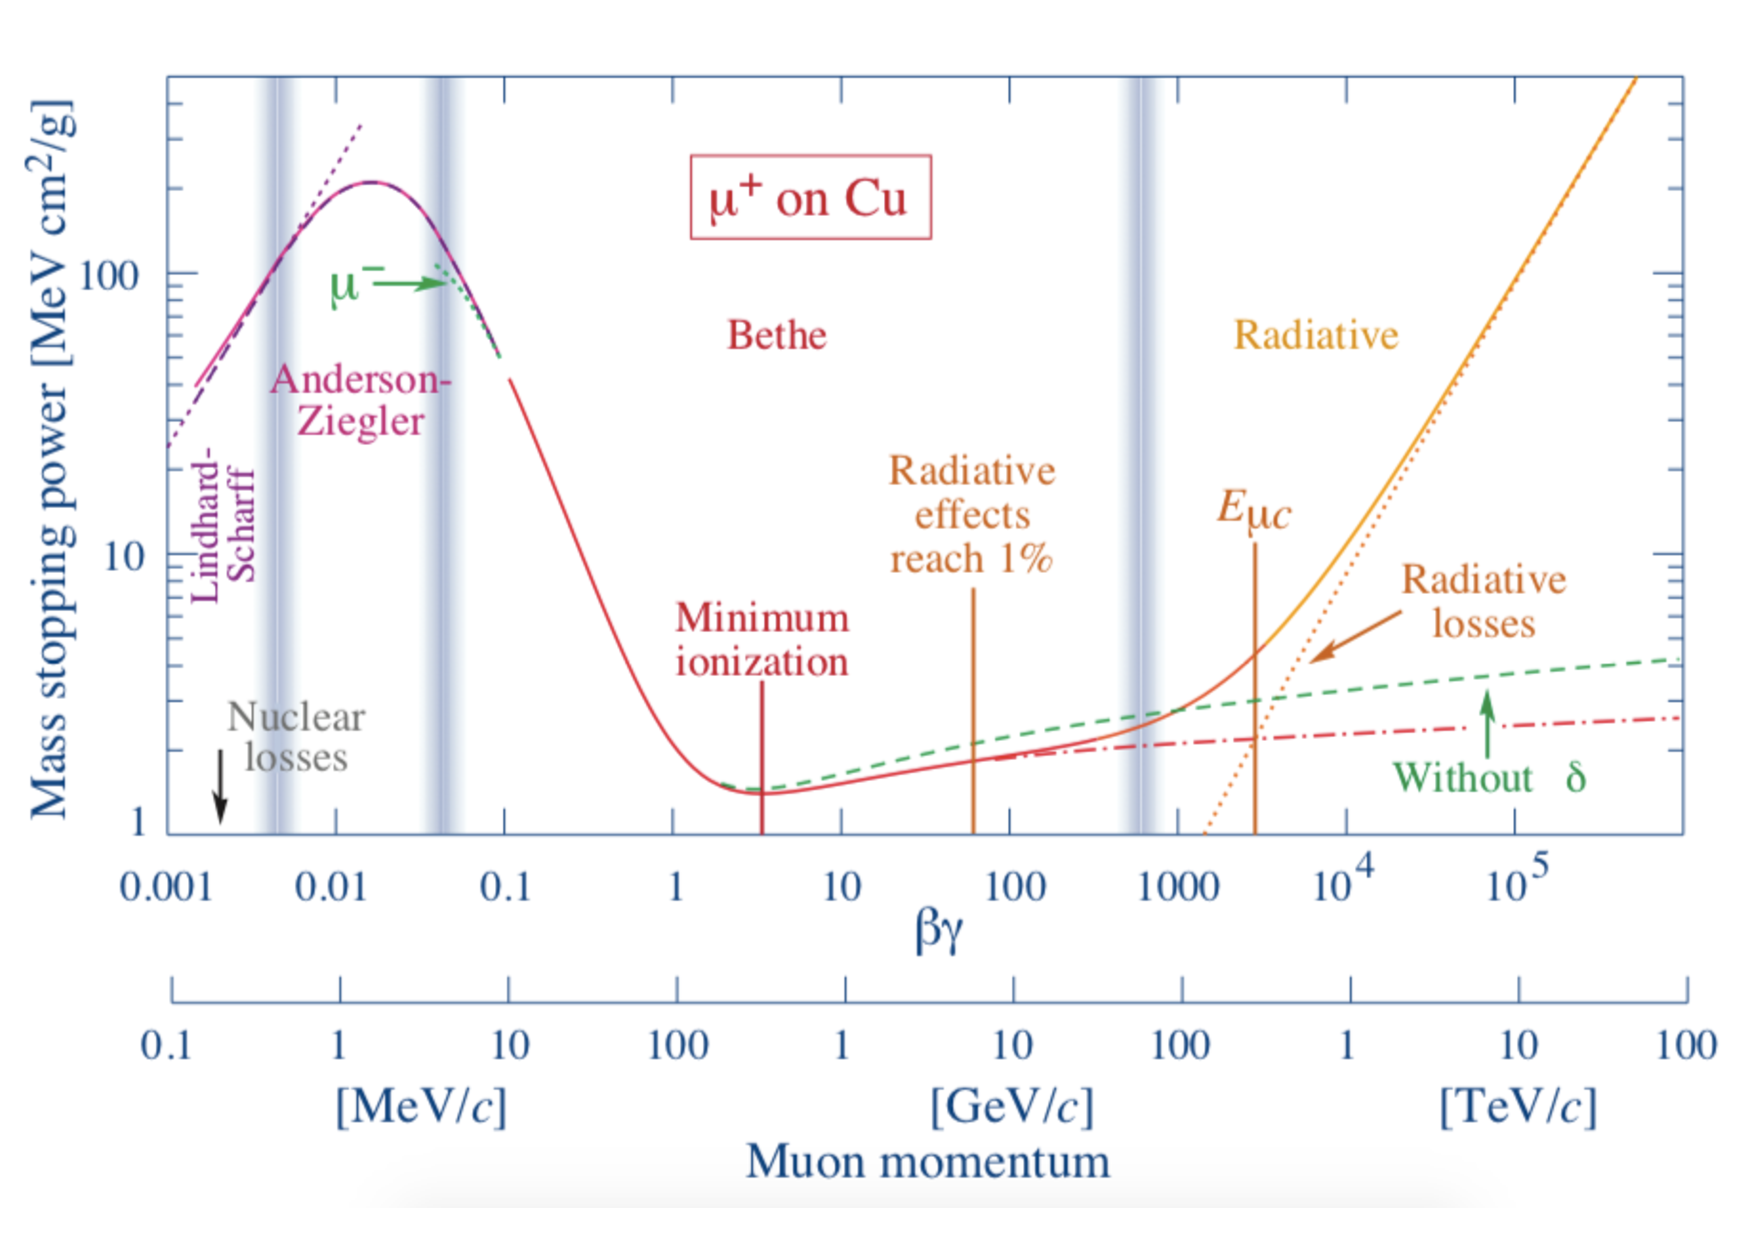
\includegraphics[width=\textwidth]{images/bethebloch.pdf}
%  \caption{Beispielhafter Verlauf des Energieverlusts für Antimyonen in Kupfer \cite{pdg}}
%  \label{fig:bethebloch}
%\end{figure}
Bei hohen Projektilenergien (relativistischen Geschwindigkeiten) entsteht ein zusätzlicher Energieverlust durch Erzeugung von Bremsstrahlung.
Außerdem gibt es weitere Korrekturfaktoren, wie die Dichtekorrektur und Korrekturen bei niedrigen Projektilenergien.
%
\\Die Wahrscheinlichkeit der Streuung von geladenen Teilchen an den gleich geladenen Atomkernen über den Raumwinkel $\Omega$ durch die Coulomb-Abstoßung wird über die Rutherfordsche Streuformel \eqref{eqn:rutherford} beschrieben.
\begin{equation}
	\frac{d \sigma(\vartheta)}{d \Omega} = \frac{1}{(4 \pi \epsilon_0)^2} \left( \frac{z Z e^2}{4 E_{\alpha}} \right)^2 \frac{1}{\sin^4{\sfrac{\vartheta}{2}}}
	\label{eqn:rutherford}
\end{equation}
Hierbei ist $E_{\alpha}$ die mittlere kinetische Energie des Projektils und $\vartheta$ der Winkel zwischen der Bahn der abgelenkten Teilchen und der Bahn der eingehenden Teilchen.
\begin{figure}[h!]
  \centering
  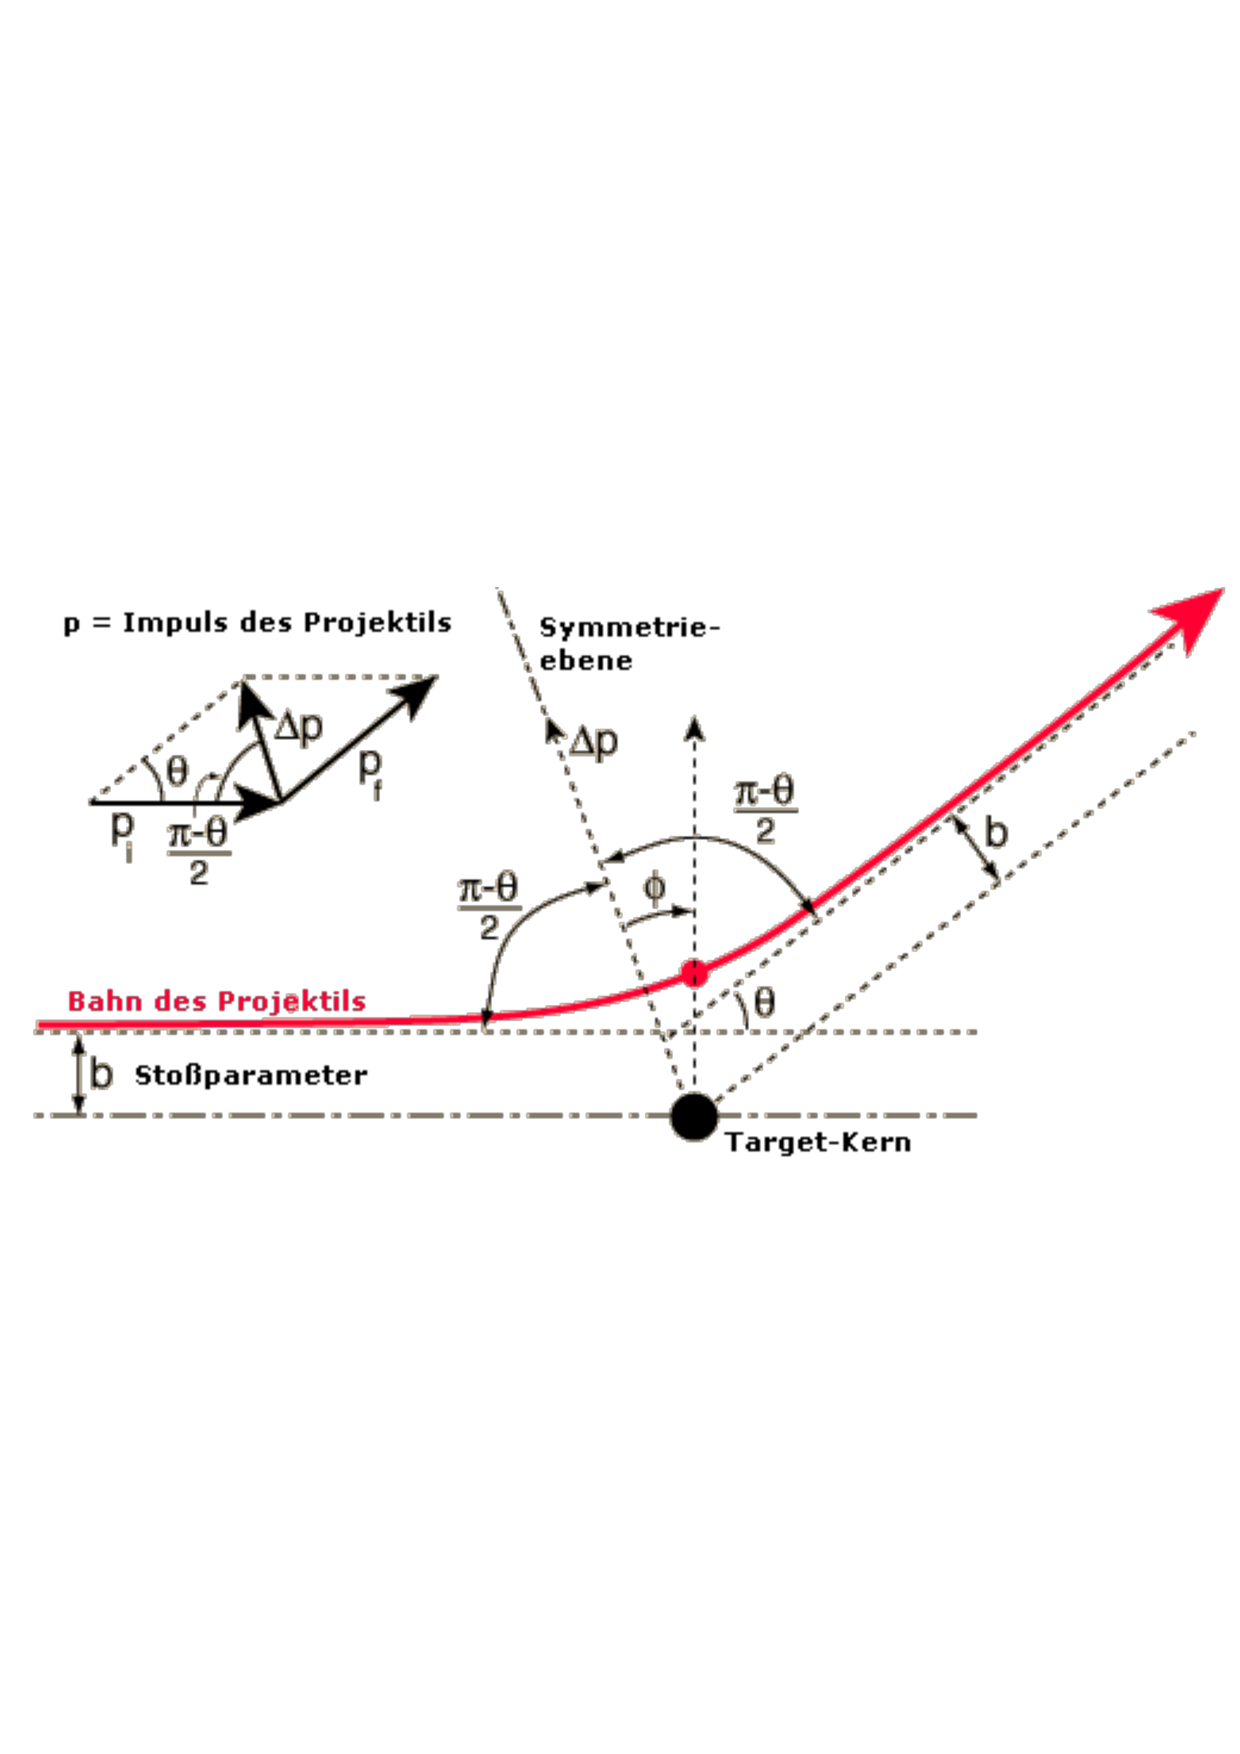
\includegraphics[width=\textwidth]{images/rutherford.pdf}
  \caption{Geometrie der Rutherford-Streuung \cite{wupp}.}
  \label{fig:rutherford}
\end{figure}
Für die Rutherfordsche Streuformel werden folgende Annahmen gemacht:
\begin{enumerate}
	\item $M_{\text{T}} >> m_{\text{P}}$, \. \. $v_{\text{P}} >> v_{\text{T}} \approx 0$: Elastische Streuung, Projektil wird abgelenkt, vernachlässigbarer Impulsübertrag an das Target.
	\item $E_{\text{kin, P}} >> V_{\text{T}}(r)$: Streupotenzial $V_{\text{T}}(r)$ ist sehr klein gegen die kinetische Energie des Projektils (Störungstheorie: Bornsche Näherung 1. Ordnung).
\end{enumerate}

%Theorie
%Wirkungsquerschnitt
%- Was ist das allgemein?
%
%Bethe-Bloch
%- Absorption von geladenen schweren Teilchen
%- Plot?
%- Formel
%- Näherungen
%
%Differenzieller Wirkungsquerschnitt
%- Herleitung?
%- Rutherfordstreuung herleiten
%- Formel
%- Näherungen
